% NeurIPS 2025 投稿模板（官方 neurips_2025.sty 已随模板附带）
% 双盲投稿用默认选项；预印本改成 \usepackage[preprint]{neurips_2025}
% 录用后改成 \usepackage[main, final]{neurips_2025}
\documentclass{article}

\usepackage{neurips_2025}

\usepackage[utf8]{inputenc}
\usepackage[T1]{fontenc}
\usepackage{hyperref}
\usepackage{url}
\usepackage{booktabs}
\usepackage{amsfonts}
\usepackage{nicefrac}
\usepackage{microtype}
\usepackage{xcolor}
\usepackage{graphicx}
\usepackage{multirow}
\usepackage{amsmath}
\usepackage{amssymb}

\title{A Compact NeurIPS 2025 Format Example\\with Figures and Tables}

\author{%
  Anonymous Author(s) \\
  Affiliation \\
  Address \\
  \texttt{email@example.com} \\
}

\begin{document}

\maketitle

\begin{abstract}
This sample demonstrates the NeurIPS 2025 single-column layout: a
centered figure, a \texttt{booktabs} table, a merged-cell table and a
numbered equation. Replace the content with your own manuscript.
\end{abstract}

\section{Introduction}
NeurIPS uses a single-column, 5.5in text width. Figures are usually
included at \verb|\textwidth| or a fraction of it, and tables follow the
\texttt{booktabs} style without vertical rules. Related work builds on
the Transformer~\cite{vaswani2017attention} and residual
networks~\cite{he2016deep}.

\section{Figures}
Figure~\ref{fig:curve} is inserted at 80\% of the text width; the
original bitmap is scaled proportionally.

\begin{figure}[h]
  \centering
  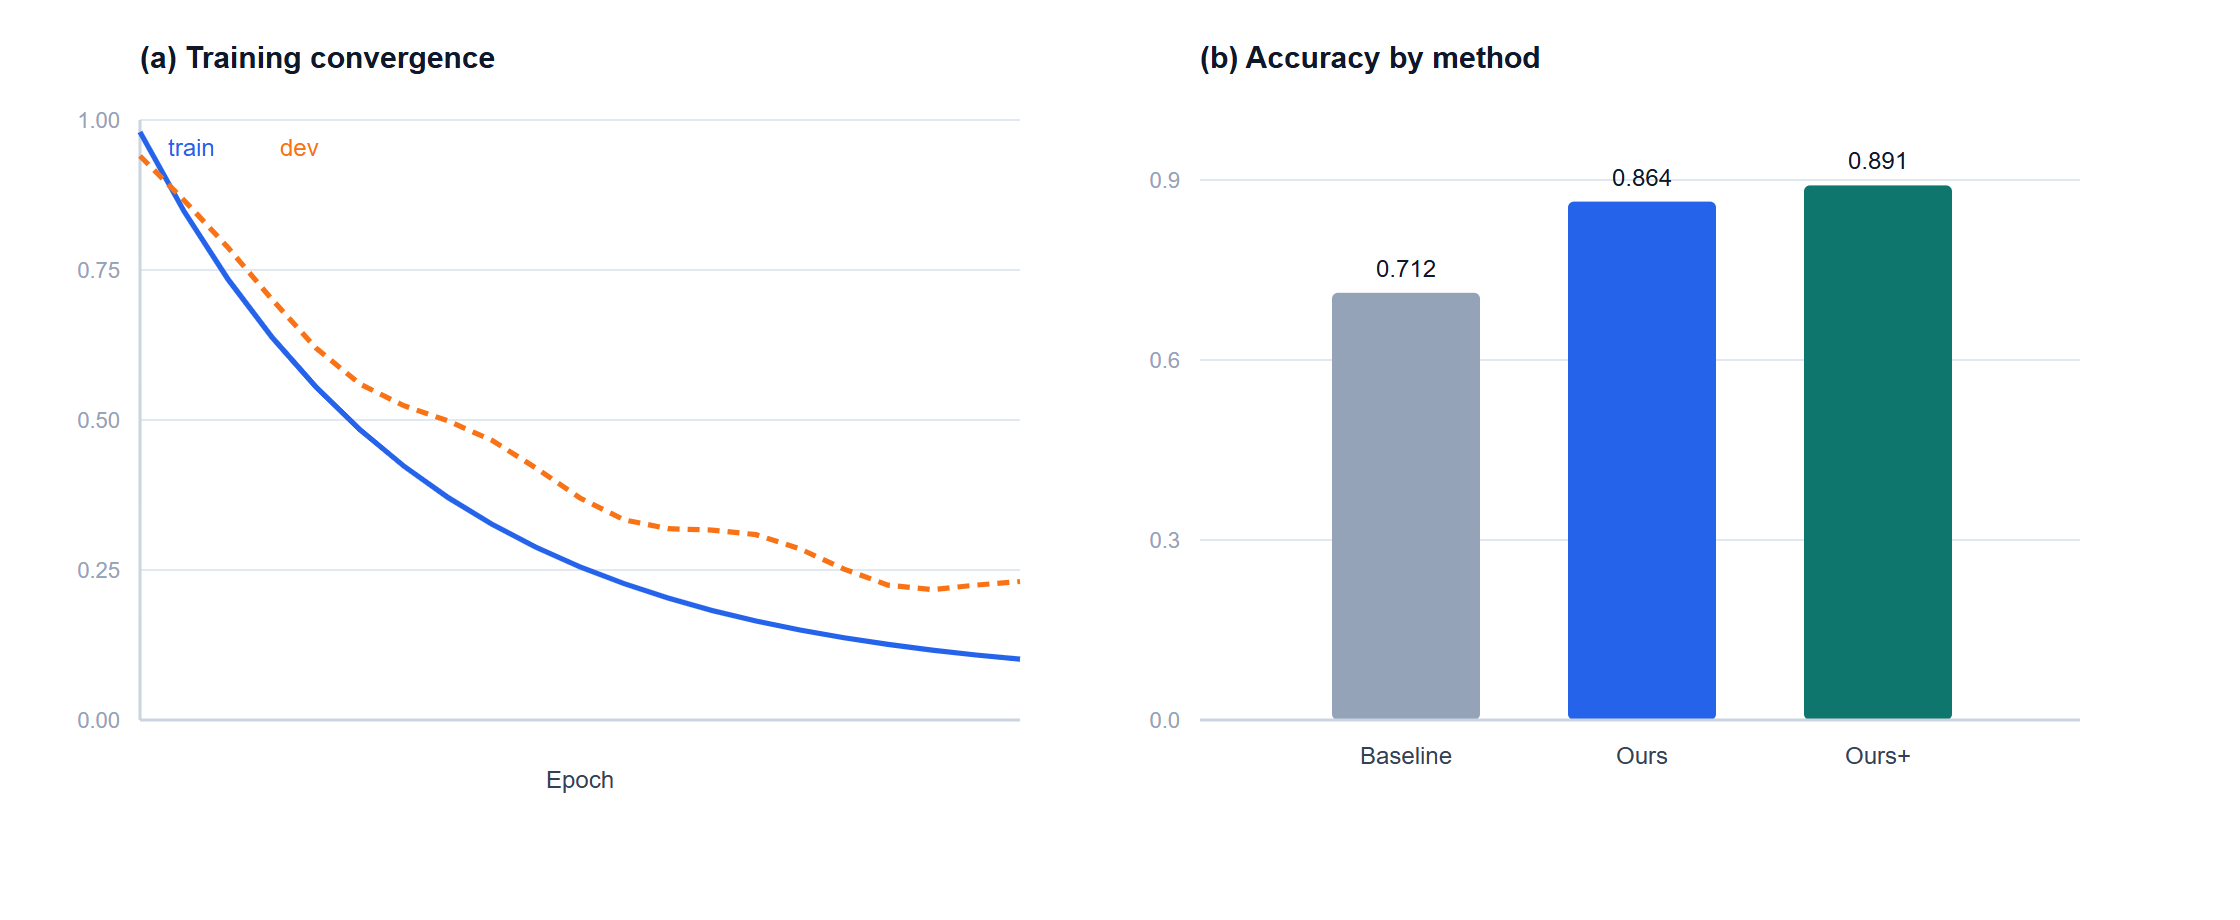
\includegraphics[width=0.8\textwidth]{figure.png}
  \caption{Training convergence and accuracy comparison.}
  \label{fig:curve}
\end{figure}

\section{Tables}
Table~\ref{tab:main} reports accuracy, and Table~\ref{tab:merged} shows
merged header cells.

\begin{table}[h]
  \caption{Accuracy of different methods.}
  \label{tab:main}
  \centering
  \begin{tabular}{lcc}
    \toprule
    Method & Dev & Test \\
    \midrule
    Baseline & 0.712 & 0.705 \\
    Ours     & 0.864 & 0.871 \\
    Ours+    & \textbf{0.891} & \textbf{0.883} \\
    \bottomrule
  \end{tabular}
\end{table}

\begin{table}[h]
  \caption{Backbone comparison with merged header cells.}
  \label{tab:merged}
  \centering
  \begin{tabular}{llc}
    \toprule
    \multirow{2}{*}{Model} & \multirow{2}{*}{Backbone} & Accuracy \\
    \cmidrule(l){3-3}
     & & (test) \\
    \midrule
    Ours  & ViT-B & 0.871 \\
    Ours+ & ViT-L & 0.883 \\
    \bottomrule
  \end{tabular}
\end{table}

\section{Equations}
Equation~\eqref{eq:gauss} is a standard display equation in the
NeurIPS text width.

\begin{equation}
  f(x)=\frac{1}{\sqrt{2\pi}\,\sigma}
  \exp\!\left(-\frac{(x-\mu)^2}{2\sigma^2}\right)
  \label{eq:gauss}
\end{equation}

\section{Conclusion}
The style file ships with this template; no additional download is
required to compile.

\bibliographystyle{plainnat}
\bibliography{refs}

\end{document}
